\section{Methoden}\label{methods}
In diesem Abschnitt wird die Funktionsweise von CRBMs beschrieben.
Grundlegendes Wissen über RBMs wird dabei vorausgesetzt.

\subsection{Convolutional RBM}\label{CRBM}
Die Convolutional RBM erweitert die normale RBM um die Möglichkeit kleine lokal auftretende Features in einem Bild zu erlernen.
Dieses Vorgehen entspricht einer Faltung wie sie in der Bildanalyse üblich ist.
Dabei besteht die CRBM aus mehreren kleinen RBMs, von denen jede jeweils einen Filter repräsentiert.
Die Größe der Filter wird zu Beginn definiert und anschließend jeder Filter mit zufälligen Werten initialisiert.
Diese Werte entsprechen den Weights zwischen den Neuronen der RBM und ein drei mal drei Pixel großer Filter entspricht dabei einer RBM mit neun Eingangsneuronen und einem Ausgangsneuron.
Jedes Bild wird mit jedem Filter gefaltet.
Dabei wird der Filter über das Bild pixelweise verschoben und die Filterantworten in eine Feature-Map geschrieben.
Für jedes Bild werden so viele Feature-Maps angelegt, wie es Filter gibt.
Die Filter-Maps sind anschließend so breit und hoch wie es Verschiebungen in x- und y-Richtung über das Bild möglich sind.

\textit{Training:}
Da die Filter zufällig initialisiert wurden müssen sie schrittweise in einem Trainingsprozess verbessert werden, um sinnvolle Features im Bild zu erkennen.
Gut trainierte Filter, sollen sich möglichst voneinander unterscheiden und die Wirkung eines Kantenfilters haben.
Somit würden verschiedene Filter auch verschiedenartige Kanten in einem Bild finden.
Der Trainingsprozess selbst besteht aus drei Schritten.
Zunächst werden die Filter $H$ auf das Originalbild $I$ angewandt und das Ergebnis jedes Filters separat in einer vorläufigen Feature-Map $R$ gespeichert.
\begin{equation*}
I * H = R
\end{equation*}
Die Filterantworten dienen dabei als Aktivierungsenergie für die Neuronen.
Diese Aktivierungsenergie wird mit Hilfe einer Logistikfunktion in eine Wahrscheinlichkeit umgerechnet, anhand derer das Neuron aktiviert oder nicht aktiviert wird.
Das Ergebnis sind die fertigen Feature-Maps.
Um das Ergebnis zu überprüfen werden Rekonstruktionen erzeugt, indem die Feature-Maps mit einem horizontal und vertikal gespiegelten Filter $fH$ erneut gefaltet werden.
\begin{equation*}
R * fH = I'
\end{equation*}
Auf die so rekonstruierten Bilder $I'$, werden die Faltungen $H$ wieder angewandt, um anschließend die Ergebnisse der rekonstruierten Daten $R'$ mit den Ergebnissen der Originaldaten $R$ zu vergleichen.
\begin{equation*}
I' * H = R'
\end{equation*}
Das Ergebnis aus dem ersten Schritt $R$ wird als Filter auf das Bild $I$ und das Ergebnis des letzten Schritts $R'$ auf die rekonstruierten Daten angewandt.
\begin{equation*}
I * R = C
\end{equation*}
\begin{equation*}
I' * R' = C'
\end{equation*}
Die Ergebnisse ($C$ und $C'$) werden subtrahiert und bilden damit den Rekonstruktionsfehler $E$.
\begin{equation*}
C - C' = E
\end{equation*}
Der Fehler $E$ wird auf den Original-Filter $H$ addiert, um ihn zu verbessern.
In der nächsten Epoche wird dann der aktualisierte Filter (H') verwendet.
\begin{equation*}
H + E = H'
\end{equation*}
Dieser Schritt nennt sich "`Contrastive Divergence"'.

\subsection{Max-Pooling}
Beim Max-Pooling handelt es sich um eine Technik der Unterabtastung, die die jeweilige Feature-Map in Regionen mit einer festgelegten Gittergröße gliedert. 
Dabei wird nur der maximale Wert der aktuellen Region übernommen.
So werden die Ergebnisdaten um den Faktor der Gittergröße reduziert und nur die maximalen Ausschläge der gelernten Filter in der Feature-Map gespeichert.
Es ergibt sich dadurch ein beabsichtigter Nebeneffekt einer Translationsinvarianz korrelierend zur Gittergröße des Max-Poolings. Durch die eingestellte Gittergröße des Max-Poolings geht die Information verloren, an welcher Stelle innerhalb des Pooling-Fensters der jeweilige Filter den Maximalwert ausgelöst hat.\newline
\begin{equation*}
\begin{matrix}
 0 & 0 & 6 & 4 \\
 0 & 1 & 7 & 3 \\
 1 & 2 & 5 & 1 \\
 0 & 0 & 3 & 0
\end{matrix} =
\begin{matrix}
 1 & 7 \\
 2 & 5  
\end{matrix}
\end{equation*}
In dem dargestellten Beispiel liegt die Regionsgröße auf $2 \cdot 2$. Aus der $4 \cdot 4$ Pixel großen Feature-Map entsteht ein $2 \cdot 2$ Pixel großes Ergebnis.  


\subsection{Kaskadierung}
Um die Translationsinvarianz zu erhöhen und die Feature Maps weiter auf signifikante und wieder auftretende Strukturen zu reduzieren, können die Ergebnisse des Max-Pooling in weiteren CRBMs verarbeitet werden. 
Der Vorgang der Filterung mit anschließendem Max-Pooling kann so lange wiederholt werden, bis die Bilddaten zu klein sind, um ein weiteres Falten oder Max-Pooling vorzunehmen\ref{cascade}. In einem klassischen Convolutional Neural Network werden allerdings nur 2 Filterungs- und Max-Pooling-Einheiten verwendet.
In der letzten Kaskade sind die unterabgetasteten Feature-Maps nur noch $1 \cdot 1$ Pixel groß. Dann lassen sie sich jeweils als ein Feature Vektor eines bestimmten Bildes interpretieren.\newline
\begin{figure*}[]
                \centering
                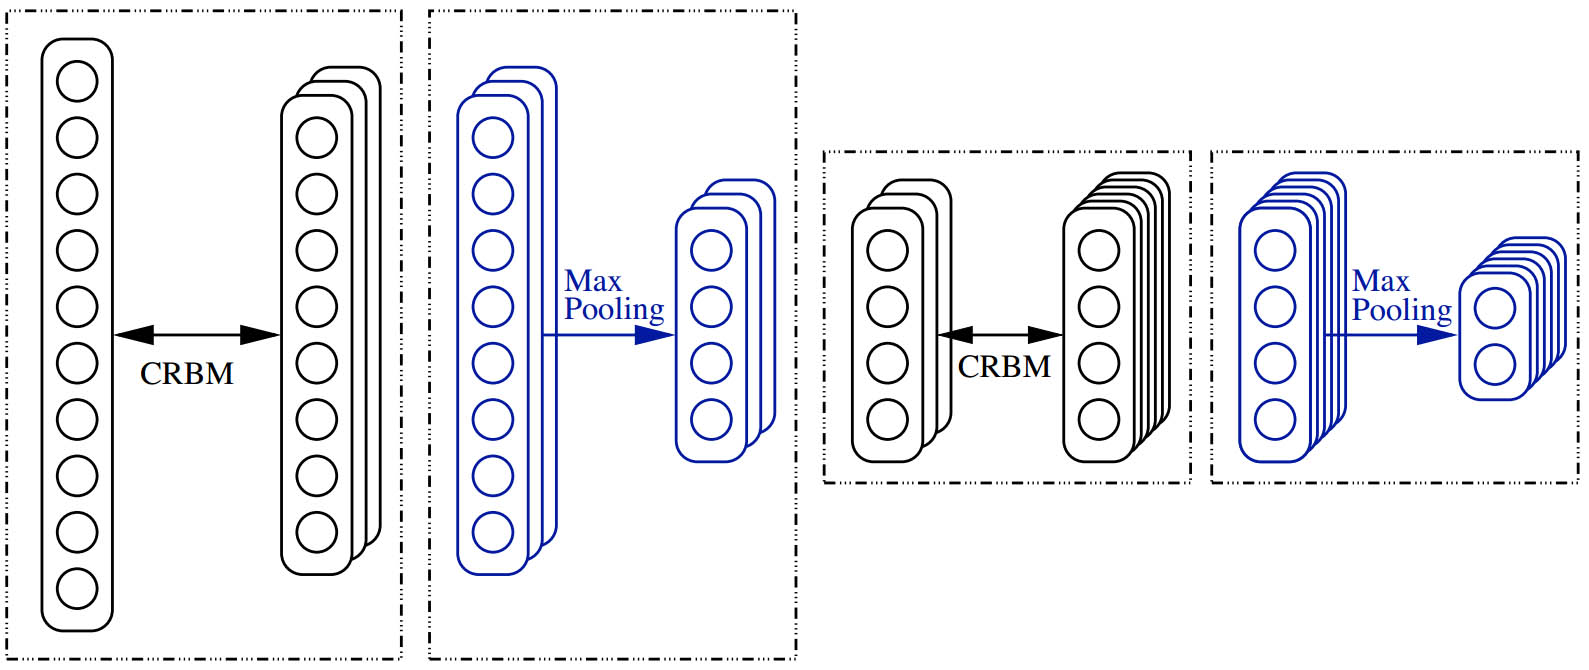
\includegraphics[width=2.0\columnwidth]{images/stack.jpg}
                \caption{CRBM-Kaskade \cite{Norouzi09}}
                \label{cascade}
\end{figure*}
